\documentclass[12pt,a4paper]{report}

\usepackage{styles/dolgozat}

\usepackage{listings}
\usepackage{styles/cpp}
\usepackage{styles/python}

\usepackage{hyperref}

\begin{document}

\pagestyle{empty} %a címlapon ne legyen semmi=empty, azaz nincs fejléc és lábléc

% A Miskolci Egyetem címere
{\large
\begin{center}
\vglue 1truecm
\textbf{\huge\textsc{Szakdolgozat}}\\
\vglue 1truecm

\includegraphics[width=4.8truecm, height=4truecm]{images/me_logo.png}\\
\textbf{\textsc{Miskolci Egyetem}}
\end{center}}

\vglue 1.5truecm %függõleges helykihagyás

% A szakdolgozat címe, akár több sorban is
{\LARGE
\begin{center}
\textbf{A szakdolgozat címe}
\end{center}}

\vspace*{2.5truecm}
% A hallgató neve, évfolyam, szak(ok), a konzulens(ek) neve
{\large
\begin{center}
\begin{tabular}{c}
\textbf{Készítette:}\\
Szakdolgozó Neve\\
Programtervező informatikus
\end{tabular}
\end{center}
\begin{center}
\begin{tabular}{c}
\textbf{Témavezető:}\\
Piller Imre
\end{tabular}
\end{center}}
\vfill
% Keltezés: Hely, év
{\large
\begin{center}
\textbf{\textsc{Miskolc, 2020}}
\end{center}}

\newpage


\newpage

\pagestyle{empty}

%Feladatkiiras
\begin{flushleft}
\textsc{\bfseries Miskolci Egyetem}\\
Gépészmérnöki és Informatikai Kar\\
Alkalmazott Matematikai Intézeti Tanszék\hspace*{4cm}\hfil \textbf{Szám:}
\end{flushleft}
\vskip 0.5cm
\begin{center}
\large\textsc{\bfseries Szakdolgozat Feladat}
\end{center}
\vskip 0.5cm
Gál Alexandra (CCTEV1) gazdaságinformatikus jelölt részére.\newline

\noindent\textbf{A szakdolgozat tárgyköre:} optimalizálás, c\# programozás\newline

\noindent\textbf{A szakdolgozat címe:} Optimális időbeosztás elérését segítő alkalmazás fejlesztése\newline

\noindent\textbf{A feladat részletezése:}

\medskip

\emph{A dolgozat feladatok időbeli ütemezésével foglalkozik. Azt vizsgálja, hogy feladatokra szánt időtartamok és a prioritások megadásával hogyan lehet adott szempontrendszer alapján optimális, vagy ahhoz közeli ütemezést elérni. Sorra veszi és összehasonlítja a hasonló célú alkalmazásokat. Példákkal illusztrálva bemutatja az elterjedt ütemezési módszereket. Az optimális ütemezést meghatározó alkalmazás C\# nyelven készül. A kapott eredményeket többek között Gantt diagramok formájában, WPF segítségével jeleníti meg a grafikus felületén.}

\vfill

\noindent\textbf{Témavezető:} Piller Imre (egyetemi tanársegéd) \newline

\noindent\textbf{Konzulens:} Sitkey Tamás (evosoft Hungary Kft. munkatárs) \newline

\noindent\textbf{A feladat kiadásának ideje:} 2020. szeptember 24.\newline

%\noindent\textbf{A feladat beadásának határideje:}

\vskip 2cm

\hbox to \hsize{\hfil{\hbox to 6cm {\dotfill}\hbox to 1cm{}}}

\hbox to \hsize{\hfil\hbox to 3cm {szakfelelős}\hbox to 2cm{}}

\newpage

\vspace*{1cm}  
\begin{center}
\large\textsc{\bfseries Eredetiségi Nyilatkozat}
\end{center}
\vspace*{2cm}  

Alulírott \textbf{Gál Alexandra}; Neptun-kód: \texttt{CCTEV1} a Miskolci Egyetem Gépészmérnöki és Informatikai Karának végzős Gazdaságinformatikus szakos hallgatója ezennel büntetőjogi és fegyelmi felelősségem tudatában nyilatkozom és aláírásommal igazolom, hogy \textit{Optimális időbeosztás elérését segítő alkalmazás fejlesztése} című szakdolgozatom saját, önálló munkám; az abban hivatkozott szakirodalom felhasználása a forráskezelés szabályai szerint történt.\\

Tudomásul veszem, hogy szakdolgozat esetén plágiumnak számít:
\begin{itemize}
\item szószerinti idézet közlése idézőjel és hivatkozás megjelölése nélkül;
\item tartalmi idézet hivatkozás megjelölése nélkül;
\item más publikált gondolatainak saját gondolatként való feltüntetése.
\end{itemize}

Alulírott kijelentem, hogy a plágium fogalmát megismertem, és tudomásul veszem, hogy
plágium esetén szakdolgozatom visszautasításra kerül.

\vspace*{3cm}

\noindent Miskolc, \hbox to 2cm{\dotfill} .év \hbox to 2cm{\dotfill} .hó \hbox to 2cm{\dotfill} .nap

\vspace*{3cm}

\hspace*{8cm}\begin{tabular}{c}
\hbox to 6cm{\dotfill}\\
Hallgató
\end{tabular}



\newpage

\noindent 1.

\begin{tabular}{cl}
&szükséges (módosítás külön lapon) \\
A szakdolgozat feladat módosítása& \\
& nem szükséges\\
&\\
\hbox to 4cm{\dotfill}&\multicolumn{1}{c}{\hbox to 5cm{\dotfill}}\\
dátum& \multicolumn{1}{c}{témavezető(k)}
\end{tabular}
\vskip1.5mm

\noindent 2. A feladat kidolgozását ellenőriztem:

\vskip1.5mm

\begin{tabular}{l@{\hspace*{4cm}}l}
témavezető (dátum, aláírás):& konzulens (dátum, aláírás):\\
\dotfill&\dotfill\\
\dotfill&\dotfill\\
\dotfill&\dotfill
\end{tabular}

\vskip1.5mm

\noindent 3. A szakdolgozat beadható:

\vskip1.5mm

\begin{tabular}{@{\hspace*{1.3cm}}c@{\hspace*{2.1cm}}c}
\hbox to 4cm{\dotfill}&\multicolumn{1}{c}{\hbox to 5cm{\dotfill}}\\
dátum& \multicolumn{1}{c}{témavezető(k)}
\end{tabular}

\vskip1.5mm

\noindent 4.
\begin{tabular}[t]{@{}l@{\hspace*{1mm}}l@{\hspace*{1mm}}l@{}}
A szakdolgozat& \hbox to 3.5cm{\dotfill} &szövegoldalt\\
              & \hbox to 3.5cm{\dotfill} &program protokollt (listát, felhasználói leírást)\\
              &\hbox to 3.5cm{\dotfill}   &elektronikus adathordozót (részletezve)\\
              &\hbox to 3.5cm{\dotfill} & \\
              &\hbox to 3.5cm{\dotfill} &egyéb mellékletet (részletezve)\\
              &\hbox to 3.5cm{\dotfill} &\\
\end{tabular}
\newline tartalmaz.

\vskip1.5mm

\begin{tabular}{@{\hspace*{1.3cm}}c@{\hspace*{2.1cm}}c}
\hbox to 4cm{\dotfill}&\multicolumn{1}{c}{\hbox to 5cm{\dotfill}}\\
dátum& \multicolumn{1}{c}{témavezető(k)}
\end{tabular}

\noindent 5.

\begin{tabular}{ll}
&bocsátható\\
A szakdolgozat bírálatra& \\
& nem bocsátható\\
\end{tabular}

\vskip1.5mm

\noindent A bíráló neve: \hbox to 8cm{\dotfill}

\vskip4mm

\begin{tabular}{@{\hspace*{1.3cm}}c@{\hspace*{2.1cm}}c}
\hbox to 4cm{\dotfill}&\multicolumn{1}{c}{\hbox to 5cm{\dotfill}}\\
dátum& \multicolumn{1}{c}{szakfelelős}
\end{tabular}

\noindent 6.
\begin{tabular}[t]{@{}l@{\hspace*{1mm}}l@{\hspace*{1mm}}l@{}}
A szakdolgozat osztályzata& &\\
&a témavezető javaslata:& \hbox to 3cm{\dotfill}\\
&a bíráló javaslata:& \hbox to 3cm{\dotfill}\\
&a szakdolgozat végleges eredménye:& \hbox to 3cm{\dotfill}
\end{tabular}

\vspace*{4mm}

\noindent Miskolc, \hbox to 4.5cm{\dotfill} \hspace*{2.5cm}
\begin{tabular}[t]{cc}
\hbox to 6cm{\dotfill}\\
a Záróvizsga Bizottság Elnöke
\end{tabular}


\cleardoublepage
\pagenumbering{gobble}
\tableofcontents
\cleardoublepage
\pagenumbering{arabic}

\newpage

\pagestyle{fancy}

\Chapter{Bevezetés}

Egyetemistaként sokszor találkozhatunk azzal a problémával, hogy alkalomadtán a világ összes ideje sem lenne elég ahhoz, hogy befejezzünk egy-egy beadandót határidőre, megtanuljuk a tananyagot a vizsga napjára vagy éppen eleget aludjunk az előbb felsoroltak teljesítése mellett. Arról nem is beszélve, hogy időnk egy jelentős részét ebben az időszakban gyakran a bulizások, diákmunka végzése vagy az állandó ingázás teszi ki a tanulás mellett. A megfelelő időbeosztás kialakításának kérdése tehát releváns szerepet játszik a hallgatók életében.

Manapság számos módszer áll rendelkezésre, amely hozzájárul feladataink hatékony rendszerezéséhez és a hatékony munkavégzéshez. Ilyen például az Eisenhower mátrix vagy a Pomodoro technika, de számtalan alkalmazás is készült már erre a célra. Ezek az alkalmazások azonban automatikus rendszerezésre nem alkalmasak, csupán egy felhasználói felületet nyújtanak feladatok nyilvántartásához és kezeléséhez.

A szakdolgozatom célja egy olyan alkalmazás készítése, amely egy optimális időbeosztás kialakítását segíti, mely által szabadidőnket a leghatékonyabban használhatjuk ki. Ennek elérése érdekében megvizsgálom a hasonló alkalmazásokat és az elterjedt hatékonyságnövelő módszereknek is utána járok. A megvalósítás során olyan ütemezési módszer felhasználását részesítem előnyben, amely figyelembe veszi és megfelelően kezeli a feladatok fontossága mellett a rájuk szánt időtartamokat is.
\Chapter{Hatékonyságnövelő módszerek}

A témám kifejtése előtt érdemesnek tartom átnézni azon módszereket, amelyek hozzájárulnak a hatékony időbeosztás megvalósításához, illetve a már meglévő alkalmazásokat, hogy azok milyen funkciókat látnak el. De mit is takar ez az egész időgazdálkodás pontosan és miért van erre szükség?

Az időgazdálkodás a rendelkezésünkre álló idő felhasználására vonatkozó döntések meghozatala, a legfontosabb teendőink elvégzéséhez szükséges idő biztosítása, továbbá a kapcsolatos információk és iratok kezelése, valamint rendelkezésre állásuk biztosítása. (http://docplayer.hu/25267846-Az-idogazdalkodas-alapjai.html) A jó időgazdálkodás lehetővé teszi, hogy ne keményebben, hanem okosabban dolgozzunk.

% TODO: (https://www.mindtools.com/pages/article/newHTE_00.htm)

Két tévhit is működik bennünk az idővel kapcsolatban. Az egyik az, hogy valamikor, egyszer, a jövőben több időnk lesz. A másik pedig az, hogy időt tudunk megtakarítani.  Valójában azonban nem megtakarítjuk, azaz csökkentjük magát az időt, az idő akkor is eltelik, ha nem teszünk semmit, és akkor is, ha sokat teszünk. Amit befolyásolni tudunk: hogyan, milyen tevékenységekkel töltjük el időnket, és azt is, hogyan éljük meg azokat a dolgokat, amelyekre időt fordítunk. 

% TODO: (Hatékony időgazdálkodás - Tananyagszerző: Máthé Judit)

Miért jó az időgazdálkodás?

Számos tanulmány kimutatta, hogy a legjobban megfizetett és a ranglétrán leggyorsabban emelkedő emberek mind-mind rendelkeznek egy tulajdonsággal, amit úgy hívnak, hogy "cselekvésorientáltság". Minden cselekvésüket áthatja ez a szemlélet. A sikeres és hatékony emberek azok, akik mindig rögtön a fontos feladatokkal kezdenek foglalkozni, és addig nem hagyják ezt abba, amíg be nem fejezték az adott feladatot. (Brian Tracy - Személyes hatékonyság c. könyve alapján)
Tehát, megállapíthatjuk, hogy életünkben jelentős előnyei vannak időnk megfelelő menedzselésének, mint például:
\begin{itemize}
\item a nagyobb produktivitás és hatékonyság elérése,
\item jobb szakmai hírnév,
\item kevesebb stressz,
\item nagyobb valószínűség az előrelépésre,
\item nagyobb valószínűség az élet- és karriercélok elérésére,
\item a mindennapi kötelezettségek könnyebb összeegyeztetése.
\end{itemize}

% TODO: (https://www.mindtools.com/pages/article/newHTE_00.htm)

\Section{Hatékonyságnövelő módszerek}

Nem újkeletű téma az, hogy hogyan lehet több időt nyerni magunknak; a régi időkben is sokakat foglalkoztatott már ez a kérdés. Számtalan módszert dolgoztak ki, megannyi technikáról olvashatunk ezzel a témakörrel kapcsolatban. A következőkben ezek közül tekintek át néhány ismertebb megoldást.

\SubSection{Eisenhower módszer}

Az egyik legismertebb technikát, az Eisenhower módszert - más néven prioritás mátrixot -, Dwight D. Eisenhower korábbi amerikai elnök dolgozta ki. Lényege, hogy teendőinket fontosságuk és sürgősségük alapján kategorizáljuk be.

% TODO: Táblázatot beszerkeszteni a forrás alapján! https://www.eisenhower.me/eisenhower-matrix/ ..és behivatkozni majd.

Négy csoportot kapunk így, amelyekhez külön utasítások társulnak.
\begin{itemize}
\item Az első negyed a „Csináld meg” kategória, amely azokat a feladatokat tartalmazza, amelyek fontosak és amiket szükséges még aznap, vagy legkésőbb másnap megcsinálni.
\item A második negyed a „Tervezd be” kategória. Ide tartoznak azok a feladatok, amelyek fontosak, viszont kevésbé sürgősek. Ezeket célszerű betáblázni a közeljövőbe.
\item A harmadik negyed azon feladatoknak van fenntartva, amelyeket delegálhatunk, mivel számunkra kevésbé fontosak, de még mindig elég sürgősek. Érdemes nyomon követni ezeket a megbízásokat, hogy később megbizonyosodjunk előrehaladásukról.
\item A negyedik és egyben az utolsó negyed a „Töröld” kategória. Ide tartoznak, azok a feladatok, amelyekkel egyáltalán nem kéne foglalkozni. Ilyenek lehetnek a rossz szokások, például a felesleges internetezéssel való időtöltés.
\end{itemize}
 
\SubSection{Pomodoro technika}

A Pomodoro technika lényege, hogy miután kiválasztottunk egy feladatot, amin dolgozni szeretnénk, 25 percig csak arra fókuszálunk. Miután letelt ez az időtartam, 5 perc szünetet tartunk, majd kezdődhet a következő intervallum. 4 periódus után pedig egy hosszabb, 20-30 perces pihenőidő ajánlott, mielőtt újra munkába lendülnénk.

A Pomodoro sokak körében ismert és használatos hatékonyságnövelő módszer, amely segít abban, hogy egy adott feladatra koncentráljunk és azt teljesítsük, viszont a szakdolgozatomban a heti szintű előretervezés a cél, így nem tartom célszerűnek erre a technikára több figyelmet fordítani.

\SubSection{GTD}

David Allen Hatékonyságnövelés stresszmentesen c. könyv alapján
A Getting Things Done (röviden GTD) módszerét David Allen tanácsadó ismerteti Hatékonyságnövelés stresszmentesen című könyvében. A munkafolyamat 5 lépésből áll, ezek a következők:
\begin{enumerate}
\item Rögzítés
\item Tisztázás
\item Rendszerezés
\item Reflektálás
\item Cselekvés
\end{enumerate}

A rögzítés lépése arra szolgál, hogy ne kelljen mindent állandóan észben tartanunk. Ennélfogva rögzítenünk kell valamilyen módon – akár írásos, akár digitális formában - minden feladatot, amelyet meg kell csinálnunk.

A tisztázás lépését az alábbi ábra szemlélteti.

% TODO: Az alább említett ábrából csinálni egy saját változatot, de behivatkozni a könyvet is!

David Allen Hatékonyságnövelés stresszmentesen 67. oldal

Ha van egy adott „dolog”, elsősorban meg kell győződnünk arról, hogy van-e vele valami teendőnk vele. Ha nincsen, akkor eldöntjük, hogy szemétbe dobható-e, később lesz-e vele valami teendőnk, vagy pedig potenciálisan hasznos információt tartalmaz, amely később még szükséges lehet számunkra.

Amennyiben az adott dologgal kapcsolatban van teendőnk, akkor három lehetőség közül választhatunk. Ha egy teendő két percnél kevesebb időt vesz igénybe, célszerű abban a pillanatban elvégeznünk, amelyben döntünk róla. Ha tovább tart, mint két perc, fel kell tennünk magunkban a kérdést miszerint mi vagyunk-e a legalkalmasabbak erre a feladatra, és ha nem, akkor érdemes egy megfelelő emberre átruházni a feladatot. Ha két percnél hosszabb időt vesz igénybe az adott tevékenység, és mi vagyunk rá a legalkalmasabbak, akkor vagy későbbre halasztjuk vagy a következő lépésre ugrunk a munkafolyamatunkban, tehát amint lehet megcsináljuk.

Érdemes megfigyelni, hogy alapjaiban véve az Eisenhower módszerhez hasonló megközelítések merülnek fel itt is. Elvégre megjelenik a delegálás, továbbá annak mérlegelése, hogy valamit betervezzünk-e a későbbiekre, vagy kezdjünk el vele az adott pillanatban foglalkozni.
A rendszerezés lépése a dolgaink feldolgozásában és értékelésében segítenek, hiszen fontos, hogy fizikai formában is tároljuk és láthatóvá tegyük a különböző kategóriákba tartozó elemeket.

A reflektálás lényege, hogy átnézzük és aktualizáljuk hetente a listáinkat, így azok folyamatosan rendszerezve legyenek, naprakészek maradjanak, könnyebben tudjunk fókuszban maradni.

A cselekvés pedig arról szól, hogy a felállított rendszert bizalommal használjuk, mivel minden döntésünk intuitív.

\SubSection{Kétperces technika}

A kétperces technika különállóan is megállja a helyét a hatékonyságnövelő módszerek között, de amint az előbb megfigyelhettük, a GTD módszerben is hasznosították ezt a stratégiát, megerősítve ezzel azt, hogy a rövidebb idő alatt elvégezhető feladatok sokat nyomnak a latban a prioritási tényező mellett.

\SubSection{Ivy Lee}

% TODO: https://www.businessinsider.com/ivy-lee-method-productivity-2018-9

Ivy Lee módszere egészen 1918-ig nyúlik vissza, amikor is Charles M. Schwab a cége hatékonyságának növelése érdekében alkalmazta őt. A 100 éves stratégia azon alapszik, hogy minden este leírjuk a 6 legfontosabb feladatot, amint másnap el szeretnénk végezni és prioritásuk szerint megjelöljük őket. Másnap a feladatoknak egyesével kezdünk neki; amikor végeztünk eggyel, akkor lépünk a következőre. A stratégia azért működőképes, mert csökkenti az egyszerre túl sok döntés meghozatalával járó nehézségeket és az időspóroláson kívül segít céljaink priorizálásában is.

Nyilvánvalóan, beszélhetnénk még olyan alternatívákról/opciókról, mint a kanban rendszer, a Zen To Done, a POSEC, Pareto 80/20-as szabálya, mindazonáltal egyértelműen megállapítható, hogy a két alappillér, a prioritás és az idő értéke az, amely szerepet játszik a minél hatékonyabb időbeosztás elérésben.


% TODO: (https://szendreiadam.hu/tervezes/idogazdalkodas-modszerek/ - csak ötletek, kifejtés máshonnan, kell-e hivatkozni majd?) -> Szét kell nézni, hogy neki mi a forrása, de egyébként lehet innen is.

\Section{Hatékonyságnövelő alkalmazások}

A különböző módszerek mellett nem szabad elfelejtkeznünk arról, hogy tennivalóink rendszerezésének megkönnyítésére mára már számos alkalmazás és applikáció létrejött. Ezek többsége azért hasznos, mert nem papír alapú, így könnyen tervezhető, átlátható és többségüket magunknál hordozhatjuk 0-24-ben. Ezek közül a legismertebbeket vesszük most számon, hogy megállapítsuk a mai appok milyen mértékben alkalmazzák az előző pontokban említett módszereket és hogyan járulnak hozzá a rendszerezéshez és hatékonyságnöveléshez.

\SubSection{Evernote}

Vitathatatlan, hogy napjaink egyik legismertebb hatékonyságnövelő alkalmazása az Evernote. Alapjáraton ez az alkalmazás nem kifejezetten csak to-do list-ek készítésére használatos, de megoldható vele feladatlisták létrehozása, amelyekhez emlékeztetőket tudunk beállítani és a checkbox-ok lehetőséget adnak az elvégzett teendők megjelölésére. Hátránya, hogy naptár funkciót nem tartalmaz és a szinkronizálás megoldása (pl. más naptár alkalmazásokkal) se egy egyszerű történet, viszont lehetőségünk van különböző sablonok felhasználására, amik között ma már találunk napi, heti, havi és évi tervező sablonokat, de akár szokáskövetőt is. Érdemes lehet megemlíteni, hogy a sablonok között találunk GTD kategóriát is.

\SubSection{Trello}

A Trello egy olyan alkalmazás, amely kimondottan a személyes hatékonyság és az időgazdálkodás javítására szolgál. Különböző úgynevezett Trello-táblákat hozhatunk létre, kiválasztva a számunkra legmegfelelőbb módszert céljaink elérésére.

A személyes termelékenységi rendszer egy heti feladatrendszerező megoldás, amely segít a feladatlisták kézbentartásában és teendőink áttekintésében.

Használhatjuk az Eisenhower mátrix tábláját is, amely az előző pontokban bemutatott módszert alkalmazza, mely segítségével minden feladat és teendő priorizálható fontosság és sürgősség szempontjából. Ez a tábla segít a hosszú távú célokon tartani a fókuszt, kiszűrve a figyelmet elterelő feladatokat, amelyek miatt nincs idő a lényegi munkára.

A heti felülvizsgálati folyamat során feladatainkat a Teendők, a Folyamatban és a Kész listák használatával tervezzük meg. A heti áttekintő ellenőrzőlisták alkalmazásával könnyedén követhetők a legfontosabb célok és az elért eredmények áttekintése. Ez az alkalmazást David Allen, a GTD módszer megalkotója is ajánlja.

% TODO: hivatkozás: https://trello.com/teams/personal-productivity

\SubSection{Google Calendar}

% TODO: A Google Keep-et is érdemes említeni!

A Google Naptár egy általam is használt és kedvelt alkalmazás. Lehetőségünk adódik akár napi, heti vagy havi nézetben áttekinteni eseményeinket és teendőinket. Adott időpontra vagy egész napra vonatkozóan adhatjuk meg az eseményeket, színjelöléseket használhatunk, és úgynevezett saját naptárakat is alkothatunk, ha egy külön projekthez szeretnénk eseményeket rendelni. Ezeket a naptárakat láthatóvá és nem láthatóvá tehetjük, így külön csoportokban jól áttekinthetővé válik minden esemény. Emlékeztetőket és feladatokat lehet létrehozni, az emlékeztetőknél beállítható az ismétlődés naponta, havonta vagy évente, a feladatokhoz pedig megjegyzéseket csatolhatunk.

\SubSection{Todoist}

A Todoist rendszere önmagában is működőképes, de összeköthető az Evernote-tal, a Trello-val, a Google Calendar-ral és egyéb programokkal is. Funkciói közé tartozik a projektek létrehozása, amikhez feladatokat társíthatunk, projektekbe ágyazott projekteket hozhatunk létre, ha több szálon futó munkáról van szó, illetve határidőket és emlékeztetőket állíthatunk be. Természetesen adhatunk meg prioritást és a színkódolás is megjelenik. Az alkalmazást gyakran használják a GTD elveire építve.

% TODO: hivatkozás: https://www.thecoffeebreak.hu/todoist-bemutato/

A Microsoft To-do segít abban, hogy a különböző tevékenységeket egy helyen vezessük. A szerteágazó feladatok rendszerezésére külön listákat alkothatunk, és ezeket meg tudjuk osztani akár családtagokkal, akár csapattagokkal. Ütemterveket tudunk készíteni, feladatokat kiosztani egy-egy csapattagnak, így nyomonkövetve a tevékenységek folyamatának alakulását.

% TODO: Megnézni, hogy hogy hivatkozható: https://www.youtube.com/watch?time_continue=121&v=-1yH5I7jdvs&feature=emb_title

Az alkalmazások táblázatos összehasonlítását az alábbi ábra mutatja.

% TODO: Az összehasonlító táblázatot beszerkeszteni!

Megfigyelhető, hogy az alkalmazások egy része vagy egy adott hatékonyságnövelő módszerre épül, vagy lehetőségünk van bizonyos szinten megvalósítani, felhasználni benne valamelyiket. A fenti áttekintésből látható az is, hogy funkciók tárháza áll rendelkezésre a rendszerzés megkönnyítése érdekében, de egyik sem nyújt olyan szolgáltatást, amely segítené felhasználóit abban, hogy tippeket adjon a hatékonyabb rendszerezésre vagy automatikusan a legjobb, legoptimálisabb időbeosztást ajánlja fel matematikai képletek vagy számítások alapján. Mivel szakdolgozatomban ezt szeretném megvalósítani, szükséges lesz valamilyen ütemezésre, amelyet a későbbiekben részletezek, de mindenekelőtt a szükséges funkciókat veszem sorra.

\Chapter{Az alkalmazás specifikációja}

\Section{Általános leírás}

A dolgozat célja egy olyan alkalmazás elkészítése, amely különböző feladatok időbeli ütemezésével foglalkozik. Az alkalmazás egy 8 órás időegységen belül vizsgálja, hogy a feladatok prioritása és a feladatokra szánt időtartamok megadásával hogyan lehet adott szempontrendszer alapján optimális, vagy ahhoz közeli ütemezést elérni. Figyelembe veszi a maximum időkeretet, így az elhanyagolható tevékenységeket kiszelektálja és a hatékonyabb időbeosztás elérését szolgáló tevékenységek beütemezését valósítja meg. A különböző feladatokat adataikkal együtt a hozzáadás sorrendjében vizuálisan ábrázolja, végül pedig egy ütemezett eredményt jelenít meg a grafikus felületen, azokkal az elemekkel, amelyek belefértek az adott időkeretbe az adott követelményrendszer szerint.

\Section{Feladatok}

A feladatok definiálása az egyik alapvető funkciója az alkalmazásnak, hiszen el kell tárolni a hozzá tartozó adatokkal együtt, hogy aztán eszerint az ütemezést végre lehessen hajtani. 

\SubSection{Feladatokhoz tartozó adatok}

Egy adott tevékenység meghatározásakor szükséges megadni a tevékenység nevét, a prioritását, ami jelzi, hogy mennyire fontos egy adott feladattal mihamarabb végezni, valamint azt az időtartamot, amely előreláthatólag lefedi a tevékenység hosszát.

Cím (\texttt{TaskTitle}): A feladat neve, a közeljövőben végrehajtani kívánt tevékenység egy szóval ábrázolva, pl.: bevásárlás.

Prioritás (\texttt{TaskPriority}): A prioritás megadásánál 3 lehetőség közül lehet választani. 1-től 3-ig adható meg, mennyire tartja fontosnak a felhasználó a feladat elvégzését; minél magasabb számérték megadása történik, annál fontosabbként lesz kezelve az adott feladat. Tehát, az 1-es számérték jelzi az alacsony prioritást, a 2-es számérték jelzi a közepes prioritást, a 3-as számérték pedig a magas prioritást. Prioritások használatakor bevett szokás szín szerinti megkülönböztető jelzést használni, így ebben az alkalmazásban is sor kerül erre. A megjelenítés során a diagramsáv keretének színe jelzi, hogy az adott feladathoz milyen értéket rendeltünk. Magas prioritás esetén piros, közepes esetén szürke, alacsony prioritás esetén zöld kerettel jelenik meg a grafikusan ábrázolt feladat sávja.

Időtartam (TaskDuration): A feladatokra szánt időtartamoknak a percben való megadására van lehetőség, mivel ezáltal a rövidebb, pár perces tevékenységek ugyanolyan könnyedén megadhatóak, mint a hosszabb, akár 1-2 órásak is. Mivel az ütemezés 8 órás időegységen belül történik, ezért 8 óránál, azaz 480 percnél hosszabb időtartamú esemény megadására nincs lehetőség, mivel annak beütemezésére úgysem kerülne sor.

Hasonló alkalmazásoknál megfigyelhető, hogy egy feladathoz még számos egyéb adat hozzárendelése lehetséges, például:

\begin{itemize}
	\item leírás,
	\item színjelzés,
	\item létrehozás ideje,
	\item különböző címkék csoportosításhoz,
	\item tulajdonos,
	\item csapattagok,
	\item státusz jelzés.
\end{itemize}

Ezeknél az alkalmazásoknál gyakran megfigyelhető, hogy nem feltétlen egy felhasználó számára készített programokról van szó, hanem lehetőséget nyújtanak több felhasználó számára, hogy például egy adott projektet egyidejűleg elérjenek és közösen dolgozzanak rajta. A felsorolt adatok pedig segítenek nyomon követni és átláthatóbbá tenni a csapatmunkát.

A programomban azért a prioritásokra és időtartamokra fókuszálok, mert az előző fejezetben nyilvánvalóvá vált, hogy ez a két tényező a legtöbb hatékonyságnövelő módszer alapja, emiatt ezzel tünt célszerűnek foglalkozni. A későbbiekben, amennyiben lehetőségem nyílik rá, megfontolandónak tartom egyéb tényezők figyelembevételét is, azaz, hogy hogyan tudnám súlyozni a feladatokat különböző szempontok szerint az előzőek mellett, mint például mennyire nehéz vagy épp mennyi haszonnal jár az elvégzése számunkra. 

\SubSection{Feladatok hozzáadása}

Feladat hozzáadásakor a cím, a prioritás és a feladatra szánt becsült időtartam megadása kötelező (\ref{fig:addTasks}. ábra). A három adat közül bármely kihagyása esetén egy felugró üzenet figyelmeztet a hibás érték(ek)re. Azonos nevű feladat hozzáadása nem lehetséges. Az időtartamhoz maximum 480 perc megadása áll rendelkezésre, erre fel is hívja a figyelmet egy üzenet a kurzort az időtartam felé mozgatva. A prioritásnál szintén hasonló üzenet jelzi a megadható prioritásértékeket (1-alacsony, 2-közepes, 3-magas).

\begin{figure}[h]
	\centering
	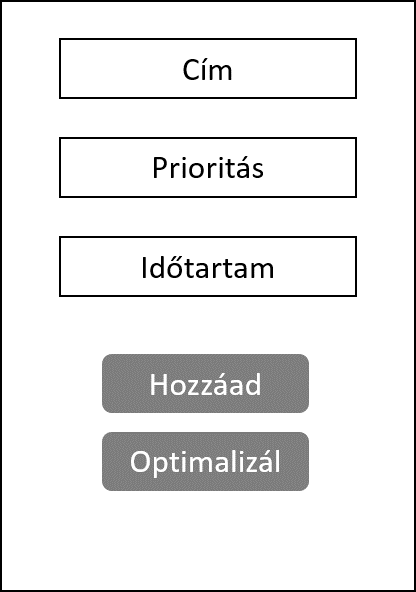
\includegraphics[scale=0.6]{images/addTasks.png}
	\caption{Feladatok definiálása a programban}
	\label{fig:addTasks}
\end{figure}

Megfelelő adatok megadása esetén, a „Hozzáad” gombra kattintva egy felugró üzenet jelzi, hogy a feladat hozzáadása sikeres volt. Ezzel egyidejűleg a feladat grafikus ábrázolása is megtörténik a diagramon. Láthatóvá kell tenni a feladat címét, mögötte a hozzá tartozó időtartammal, valamint egy, az időtartammal megegyező hosszúságú sávot, a prioritásnak megfelelő piros, szürke vagy zöld kerettel (\ref{fig:diagram}. ábra).

\begin{figure}[h]
	\centering
	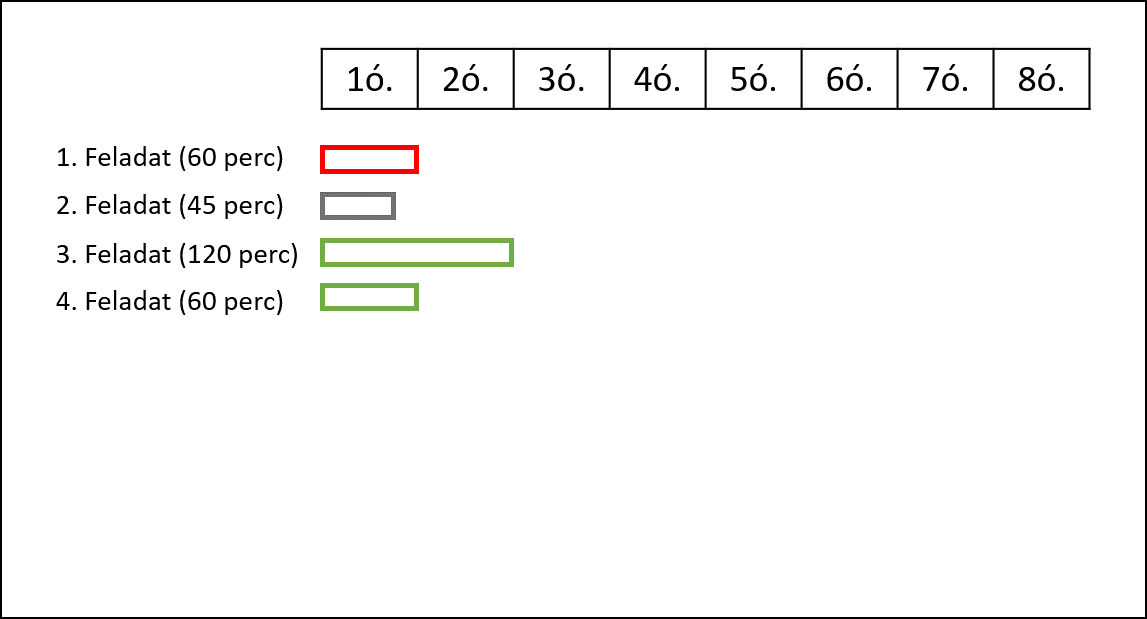
\includegraphics[scale=0.8]{images/diagram.png}
	\caption{Feladatok grafikus ábrázolása}
	\label{fig:diagram}
\end{figure}

További feladatok definiálásakor a diagramon megjelenő információk mindig az előzőek alá kerülnek.

\Section{Optimalizálás és ütemezés}

Az optimális ütemezés meghatározása és megjelenítése az alkalmazás lényegi funkciója. A feladatok ütemezése során a programnak az időkeretbe beleférő legnagyobb összértéket kell előállítania, ezáltal pedig a lehető leghatékonyabb megoldást, tervezetet megkapni. Az ütemezés kivitelezésére külön fejezetben kerül sor, ahol meghatározom magát az ütemezési problémát, valamint a lehetséges megoldásokat rá. Az optimalizálás a program futása során nem automatikusan történik, minden egyes újabb feladat hozzáadásakor, hanem a felhasználó az általa szükségesnek vélt feladatok hozzáadása után kérheti az ütemezést az "Optimalizál" gomb megnyomásával.

Az optimalizálás végrehajtásához minimum két feladat megléte szükséges. Az "Optimalizál" gomb megnyomására a program végrehajtja az optimalizálást és az ütemezést. A sikeres ütemterv létrehozását egy felugró ablak jelzi. Ezután megjelenik egy "Ütemezett sorrend" felirat, melyet követően azon feladatok nevei szerepelnek, amelyeket a program beütemezett a 8 órás időkeretbe, olyan sorrendben, ahogy azokat célszerű végrehajtani az ütemező szerint. Az ütemterv grafikus ábrázolása során a diagramon megjelenő sávok egymás mellett jelennek meg lehetőség szerint kitöltve a 8 órányi időtartamot. Az ütemező a kihagyott feladatok neveit is megjeleníti (\ref{fig:scheduledTasks}. ábra). Amennyiben az ütemezendő feladatok összideje nem éri el a 8 órát, akkor minden elem sikeresen belekerült az időkeretbe, akkor ezt egy "Minden feladat belefért az időkeretbe!" felirat jelzi.

\begin{figure}[h]
	\centering
	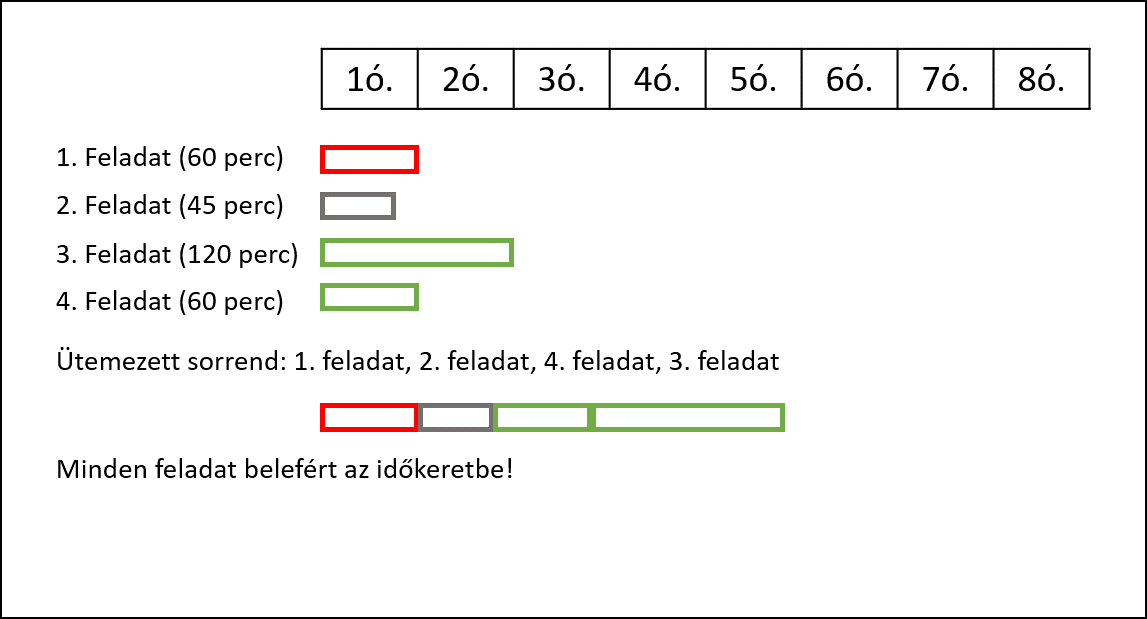
\includegraphics[scale=0.8]{images/scheduledTasks.png}
	\caption{Ütemterv grafikus ábrázolása}
	\label{fig:scheduledTasks}
\end{figure}

\Chapter{Az ütemezési probléma}

\Section{Az ütmezési probléma}

Az ütemezési probléma során azzal a kérdéssel állunk szembe, hogy milyen módon oldható meg, hogy a szabadon rendelkezésre álló feladatainkat úgy osszuk be, hogy azzal a lehető leghatékonyabb eredményt érjük el. A cél, hogy olyan időbeosztást kapjunk, ahol az ütemtervbe bekerült feladatok összértéke a legnagyobb lesz. 

Ahhoz, hogy eldöntsük a feladatok közül melyek azok, amelyeket érdemes megvalósítanunk, valamint ahhoz, hogy ezeket hatékony sorrendben elhelyezhessük, szükségünk van olyan adatokra, amelyekkel jellemezni tudjuk a tevékenységeket és olyan számításra, képletre, amely hozzájárul ezek ütemezéséhez. A dolgozatomban ezen adatok, melyek jellemzik a tevékenyégeket, a már említett prioritás és idő, valamint ezek hányadosai lesznek. 

Az ütemezés egyik fele tehát arról szól, hogy mely feladatok beütemezése által érjük el a lehető legnagyobb összértéket, tehát a legfontosabb feladatok kiválogatása, amely még belefér az időkeretbe. Itt amire figyelni kell az az, hogy ha van egy magas prioritású feladat a listánkon, ami még beleférne az időkeretünkbe, de van másik két kisebb prioritással rendelkező feladat is, amely szintén beleférne ebbe a keretbe és azok összértéke (prioritása) együttesen nézve magasabb értéket képvisel, mint az előbbi feladaté, akkor ezt a két tevékenységet helyezzük előtérbe az előbbi egy, magasabb prioritású feladat helyett.

Az ütemezés másik fele a sorrend kialakításáról szól. Itt a prioritás még mindig egy fontos tényező, de az idő is meghatározó szerepet játszik. Kétségkívül, ha egy feladat csupán pár perc alatt letudható, azt nem érdemes halogatni – ld. kétperces technika módszere -, de nem hagyható figyelmen kívül a rövid „to-do-k” miatt egy sok időt felemésztő, de magasabb értéket képivelő tevékenység sem. Emiatt a prioritás/időtartam hányados szerinti csökkenő sorrendben történő ütemezést tartom itt megfelelőnek. Eszerint, ha megegyezik az időtartam kettő vagy több feladatnál, akkor a prioritás fog előtérbe kerülni és amelyik fontosabb azt ütemezzük előrébb, míg, ha a prioriás megegyezik, de valamelyiknek rövidebb az ideje, akkor a rövidebb időtartammal rendelkező feladatot válasszuk hamarabb az ütemezés során. Abban az esetben, ha megegyeznek az időtartamok és a prioritások is, és ugyanazt a hányadost kapjuk a képlet végén, a hozzáadási sorrend szerint ütemezhetjük be őket. Megjegyezném, hogy egy későbbi, továbbfejlesztett verzióban itt adódik remek lehetőség arra, hogy a modellben ne csak az adott két hányadossal számoljunk, hanem a már említett tényezőket is figyelembe vegyük, mint például mennyi haszonnal jár vagy épp mennyire nehéz a feladat elvégzése és ezeket a számításba belekalkulálva egy még hatékonyabb megoldást érhetünk el.

Az optimalizálás és ütemezés során bementként várt értékek a programban a következőképp alakulnak majd.

Minden egyes feladahoz szükséges definiálni:

\begin{itemize}
\item egy prioritást: 1, 2 vagy 3-as értékkel, és
\item feladat elvégzéséhez szükséges becsült időtartamot: 1-480 perc között.
\end{itemize}

A sorba rendezés kialakításához ebből a két értékből kapott prioritás/időtartam hányadost használjuk fel.

Az időkeret értéke előre definiált 480 perc.

Kimenetnél egy olyan ütemtervet várunk, ahol azon feladatok kerültek beütemezésre, amelyek belefértek a 480 perces időkeretbe úgy, hogy fontosságuk a legnagyobb összértéket képviselik, mindezt a feladatokhoz tartozó prioritás/időtartam hányados alapján csökkenő sorrendben kialakítva.

A következőkben különböző lehetőségeket vizsgálok meg, amelyek segíthetnek a feladatok beütemezésében és az optimalizált eredmény elérésében.

\Section{A hátizsák feladat}

A hátizsák probléma egy dinamikus programozási probléma, amely az optimalizálási kategóriába tartozik. Célja, hogy adott súlyokkal és hozzárendelt értékekkel rendelkező elemek esetén maximalizálja az értéket egy hátizsákban, miközben a súlykorlátozáson belül marad. Minden elem csak egyszer választható ki, mivel egyetlen tételből sem áll rendelkezésünkre több mennyiség.\cite{knapsack}

A megoldás során előkészületeként feltehető, hogy az elemek érték/tömeg szerint csökkenő sorrendben vannak indexelve.

A hátizsák feladat felhasználása teljesen mértékben célravezetőnek tűnik, hiszen az érték/tömeg páros teljes mértékben megfeleltethető az általam tervezett alkalmazás prioritás/időtartam attribútumaival, és megoldja azt a problémát is, hogy úgy válassza ki az elemeket egy listából, hogy azzal eleget tegyen a kapacitás feltételének és emellett egy maximalizált eredmény adjon. Emellett a sorba rendezés problémáját is megoldja maga az optimalizálás elvégzése előtt, így nincs szükség utólagos ütemezésre.

\Section{Erőforrás tervezéshez kapcsolódó algoritmusok és szabályok}

A hátizsák feladat ugyan egy az egyben ráilleszthető az adott program matematikai modelljére, mint megoldás, de hasznosnak tartom áttekinteni más lehetőségeket is. A termelésinformatika területén belül, pontosabban erőforrás tervezés során már sokat tanulhattam magáról az ütemezésről, különböző ütemtervek megvalósításáról és a hozzá kapcsolódó algoritmusokról is. A következőkben ezek közül nézek meg néhányat. Érdemes lehet megjegyezni, hogy az erőforrás tervezés során az algoritmusok és az elvégzendő munkák lehetnek egy vagy több gépre tervezve és ezekhez tartozhatnak különböző szabályok az ütemezések célja szerint.

\SubSection{Palmer-módszer}

Elsőként a Palmer módszer jutott a témával kapcsolatosan eszembe, amely azért keltette fel a figyelmem, mert itt a munkákhoz prioritási indexet kell rendelni, és ennek a prioritási indexnek az értéke alapján történik meg az ütemezés. A prioritási index kiszámolására azonban olyan formula áll rendelkezésre, amelynek elve, hogy azok a munkák kerüljenek előre, amelyeknek a megmunkálási idői az első gépeken rövidebbek a többihez képest. Így, mivel a prioritást szimplán idő alapján számolja, valamint többgépes rendszerre érvényes módszer, el is vetettem ennek a használatát.\cite{palmer}

\SubSection{Dannenbring-módszer}

A következő, Dannenbring-módszer ugyan súlyozási sémát használ az ütemezésekhez, viszont szintén többgépes feladatoknál alkalmazható, így visszatértem más tanult módszerek megvizsgálásához, pontosabban az egyetlen erőforrást tartalmazó ütemezési feladatok megoldásaihoz és onnan próbáltam ötleteket szerezni.

\SubSection{Az SPT szabály}

Az SPT (Shortest Processing Time) szabály lényege, hogy a munkákat a műveleti idők alapján nemcsökkendő sorrendbe rendezzük és ennek megfelelően indítjuk el azokat. Ez jelen esetben nálunk azt jelentené, hogy a tevékenységeket az alapján állítanánk sorba, hogy melyikkel tudunk leghamarabb végezni, viszont így az a probléma áll majd fent, hogy a prioritással nem tudunk foglalkozni.\cite{sptwspt}

\SubSection{A WSPT szabály}

A WSPT (Weighted Shortest Processing Time) szabály a legkisebb súlyozott műveleti idejű munkát veszi előre. Itt már tehát szóba jön a súlyozás is, a munkák ideje mellett, tehát ez a módszer használhatónak tűnik. A WSPT szabály lényege, hogy minden egyes munka – a dolgozatomban feladat – esetében w/p hányadosokat képzünk, ahol a w egy J munka súlyát, a p az adott J munka műveleti idejét jelenti. Majd elrendezzük a munkákat a kapott w/p hányadosaik alapján nemnövekvő sorrendbe és ennek megfelelően indítjuk el azokat.  Tehát egy w/p fontossági mutatót kapunk és minél nagyobb lesz egy munka mutatója, annál előrébb fog kerülni a sorban.\cite{sptwspt}

A felsorolt ütemezések közül ez a szabály a sorba rendezés problémáját megoldaná, viszont arra nem elegendő, hogy figyelembe vegye mely feladatok által érhetnénk el a maximális összértéket.

A dolgozatomban végül a hátizsák feladat algoritmusának felhasználására esett a választásom, mivel a programom ütemezési és optimalizálási problémájára is hatékonyan alkalmazható.

\Chapter{Tervezés}

\Section{Felhasznált technológiák}

\SubSection{C\#}

Az egyetemi éveim alatt lehetőségem volt 2 féléven keresztül az evosoft Hungary Kft. evoCampus-án részt venni, ahol megismerkedtem a C\# nyelvvel, amelyet végül az alkalmazásom megvalósításához választottam.

A C\# egy általános célú, objektumorientált programozási nyelv, valamint a .NET egyik fő programozási nyelve. A C nyelvcsaládhoz tartozik, így ismert lehet a C++ és Java programozók számára, hiszen ilyen alapokon fejlesztették ki. Platformfüggetlenségét a .NET környezet biztosítja.

A .NET keretrendszer gyors és hatékony alkalmazásfejlesztést biztosít a .NET osztálykönyvtárak által. A különböző nyelveken írt komponensek együttműködését pedig a CLR (Common Language Runtime) és a CTS (Common Type Sytem) segítségével könnyíti meg.\cite{csharp}

\SubSection{Visual Studio}

A Visual Studio egy integrált fejlesztői környezet, amelyet a Microsoft fejlesztett ki különböző alkalmazások, pl.: konzol, webalkalmazások, mobilalkalmazások fejlesztésére. Lehetőséget nyújt a C\#-on kívül például Viusal Basic, F\# és számos más nyelveken történő programozásra.  Az alkalmazásom megvalósításakor én a Community kiadást választottam, ami egy olyan ingyenes verzió, amely a Professional kiadáshoz hasonló szolgáltatásokat tartalmaz.\cite{vs}

\SubSection{WPF}

A WPF (Windows Presentation Foundation) egy grafikus felhasználói felületet biztosító keretrendszer. Előnye a XAML nyelv, amely megkönnyíti a felhasználói felület létrehozását és szerkesztését, valamint lehetővé teszi magának a UI tervezésének elkülönítését a program többi részétől. Emellett, lehetőség van DataBinding használatára, amely állandó kapcsolatot biztosít az alkalmazás felhasználói felülete és backend-en tárolt adatok között. Így, egy adat backend-en történő értékének megváltozása során a felhasználói felület automatikusan fog frissülni és fordítva.\cite{wpf}\cite{databinding}

\SubSection{MahApps}
A MahApps egy olyan keretrendszer, amely egy modernebb felhasználói felület elérését segíti a WPF-en keresztül. Az alkalmazásom megvalósítása kezdetén kezdtem használni, viszont a későbbiekben háttérbe került a diagram Canvas-sal történő fejlesztése miatt.

\SubSection{MVVM}
Az MVVM rövidítés a Model, View, ViewModel szavakból származik. A séma lényege, hogy az alkalmazásunkat erre a három, jól elkülöníthető logikai egységre szedjük szét, mely által jobban átláthatóvá válnak. A három egység különböző célokat szolgál.

\begin{figure}[h]
	\centering
	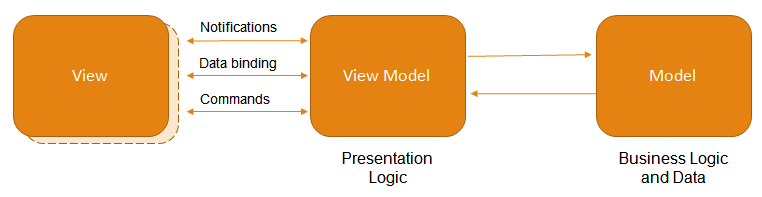
\includegraphics[scale=0.5]{images/mvvm.png}
	\caption{Az MVVM működése\cite{mvvmpic}}
\end{figure}

A View szerepe a grafikus felület biztosítása, minden, amit a képernyőn meg szeretnénk jeleníteni, azt megadhatjuk itt a XAML kód által. A XAML kódon belül definiáljuk a binding-okat is.

A Model tartalmazza a különböző adatokat és osztályokat, amikkel dolgozni szeretnénk.

A ViewModel pedig a kettő közötti kapcsolatot adja meg. Itt történik például a példányosítás, és ezáltal jeleníthetjük meg azt, amit a View-n látni szeretnénk, általában command-okon keresztül.\cite{mvvm}

\SubSection{Azure DevOps}

Az Azure DevOps (korábban Visual Studio Team Foundation Server (TFS)) szoftverfejlesztői szolgáltatásokat nyújt csapatok számára az alkalmazások készítéséhez és a projektmunka hatékony végzéséhez. Én személy szerint a verziókövetés (5.2. ábra) miatt tartottam fontosnak a használatát, mivel lehetővé teszi, hogy a kódban történő változtatásokat nyomon követhessem, engedélyezi, hogy szükség esetén egy korábbi változatra visszaálljak és nyilvántartja a különbségeket a verziók között. Különböző verziókat is összeilleszthetünk, ilyenkor a módosítások miatt felmerülő problémák esetén pedig a konfliktusok lekezelésére is lehetőség van.\cite{azure}

\begin{figure}[h]
	\centering
	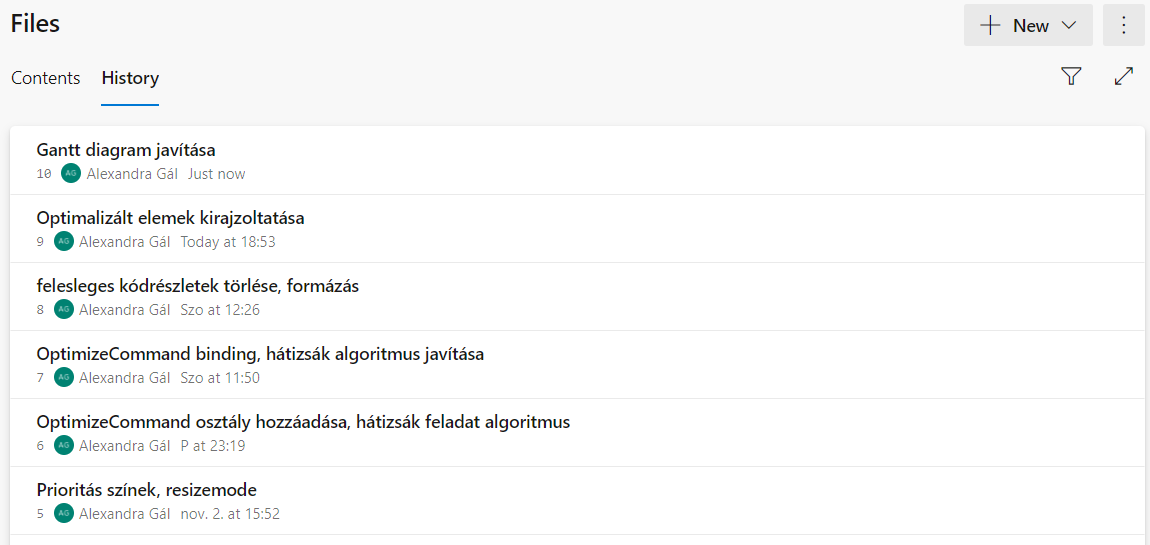
\includegraphics[scale=0.5]{images/azureHistory.png}
	\caption{Verziókövetés az Azure DevOps-ban}
\end{figure}

\SubSection{ItemsControl, Canvas, Rectangle osztály}

Mivel C\#-ban a legtöbb lehetőség a diagramokat illetően a WinForms-hoz kapcsolódik és nem a WPF-hez, vagy pedig nem nyílt forráskódú könyvtárak által lenne lehetséges, ezért úgy döntöttem, hogy a vizuális ábrázolást az ItemsControl, a Canvas, és a Shape könyvtár közül a Rectangle osztály segítségével oldom meg.

A Rectangle osztály segít a téglalapok megrajzolásában, ami a feladatok hosszát reprezentáló sávot ábrázolja majd a diagramon.

A Canvas egy olyan területet biztosít, ahol elemeket tudunk pozícionálni.

Az ItemsControl fogja tartalmazni a Canvast, amelyet az ItemsControl ItemsPanel-jére tudunk elhelyezni. Az ItemsControl-ra azért van szükség, mert a kirajzolandó téglalapok egy Rectangle típusú ObservableCollection-ben lesznek eltárolva és ez a Control a kollekciók elemeinek megjelenítését segíti.

\Section{UML diagram}

Az alkalmazás UML diagramja az 5.2. ábrán látható. A program során az MVVM és Binding használatát a Command-ok segítik. A Command osztályok kapcsolatban állnak a ViewModel-lel, ami kapcsolatot létesít a UI felület és backend adatok között. Az AddTaskCommand-ban valósul meg a feladatok példányosítása, majd ezeknek a grafikus felületen történő megjelenítése a DrawChart osztályon belüli DrawTasks metódus által történik. Az OptimizeCommand osztály szolgál a feladatok ütemezésének és optimalizálásának végrehajtásához. A sorrendkialakítás a Knapsack osztály OrderTasks metódusa által, míg az ütemezési probléma megoldására választott hátizsák algoritmus a KnapSackAlgorithm metódus által valósul meg. A végső, kialakult ütemtervet a DrawChart osztályon belül a DrawScheduledTasks metódus által jeleníti meg az alkalmazás.

Az MVVM-es megközelítés miatt a Command-okban szerepel egy-egy CanExecute metódus, amelyek után, true visszatérési érték esetén lefutnak az Execute metódusok, amelyek a végrehajtandó programkódokat -, mint például egy feladat példányosítása vagy az OrderTasks metódus meghívása - tartalmazzák. A MainViewModel által tartalmazott RaisePropertyChanged metódus szintén az MVVM fontos részeként szokott szerepelni, az INotifyPropertyChanged interfészhez és a NotifyPropertyChanged event-hez kapcsolódva, amely a UI felé történő változások értesítéséért és frissítésekért felel.

\begin{figure}[h]
	\centering
	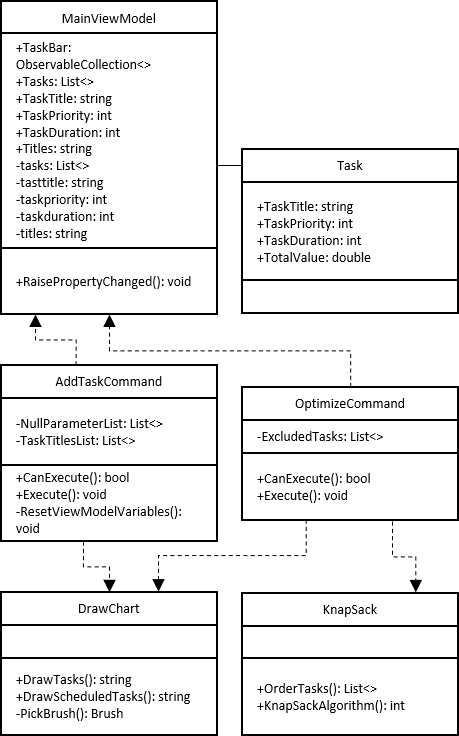
\includegraphics[scale=1.3]{images/uml.png}
	\caption{Az alkalmazás UML diagramja}
\end{figure}

\Chapter{Megvalósítás}

\Section{Feladat hozzáadása}

A feladatok hozzáadásánál mindig a három, már ismertetett értéket kell megadni, tehát a feladat címét, a prioritását és az elvégzéséhez szükséges becsült időtartamot. A prioritás és időtartam megadásánál ToolTip-pel jelzi a program a segítő információkat, minthogy a prioritás értékhez csak az 1, 2 és 3 értékek adhatóak meg, az időtartamnál pedig maximum 480 perc.

\begin{java}
<TextBox Text="{Binding TaskPriority, Mode=TwoWay}"
TextChanged="TextBox_TextChanged"
mah:TextBoxHelper.Watermark="Prioritas:"
ToolTip="1 - alacsony, 2 - kozepes, 3 - magas"
mah:TextBoxHelper.UseFloatingWatermark="True"
Margin="0 0 0 10"
x:Name="priorityTextBox"
PreviewTextInput="priority_PreviewTextInput"/>
\end{java}

Mindhárom érték átadását a binding segíti.

\begin{java}
<TextBox Text="{Binding TaskTitle, Mode=TwoWay}"
<TextBox Text="{Binding TaskPriority, Mode=TwoWay}"
<TextBox Text="{Binding TaskDuration, Mode=TwoWay}"
\end{java}

Ehhez szükséges még az AddTaskCommand definiálása, amely a „Hozzáad” című CommandButton megnyomása során fut le.

\begin{java}
<Button 
Margin="0 0 0 10"
Command="{Binding AddTaskCommand}"
CommandParameter="{Binding Text}"
Click="AddTaskButton_Click"
Height="20" Width="80"
Name="btnAddTask"
Content="Hozzaad"/>	
\end{java}

Ilyenkor a ViewModel-en keresztül kapcsolat jön létre a Command-dal. Egy Command meghívásakor többek között az Execute(object Parameter) egy paraméteres metódus fut le, ahol a Command által használt adatok kerülnek továbbításra.

Az általunk megadott adatokat eltároljuk egy Task osztály típusú változóban. A példányosítás során a Task osztály csupán 3 adata kerül beolvasásra, de ezen kívül található még egy TotalValue property is, amely automatikusan a prioritás/időtartam hányadost számolja ki. Ez a későbbiekben, az optimalizálás során kerül felhasználásra.

\begin{java}
//Task class konstruktora
public Task(string title, int priority, int duration)
{
	TaskTitle = title;
	TaskPriority = priority;
	TaskDuration = duration;
	TotalValue = (double)priority/(double)duration;
}	
\end{java}

A létrejött példányunkat végül hozzáadjuk a Task osztály típusú Tasks listánkhoz. Ez a lista tárolja majd az összes definiált task-ot.

\begin{java}
	var task = new Scheduler.Task(
	mainViewModel.TaskTitle,
	mainViewModel.TaskPriority,
	mainViewModel.TaskDuration);
	
	mainViewModel.Tasks.Add(task);
\end{java}

A példányosítás előtt még megtörténik az adatok helyes formátumban való megadásának ellenőrzése is. A Command ezáltal csak akkor fut le, ha minden érték helyesen van megadva, ellenkező esetben MessageBox-szal jelzi a hibásan megadott értékeket.

\Section{Feladat megjelenítése grafikusan}

A következő lépés a feladat vizuális megjelenítése. Ez még mindig az AddTaskCommand meghívása során történik a DrawTasks metódus segítségével. Ennek szerepe, hogy az adott task-ot grafikusan megjelenítse a UI-on egy új rectangle létrehozása által. A task tulajdonságaiból felhasználjuk az időtartamot, ami a rectangle hosszát fogja adni, és a prioritást, amivel vizuálisan is szemléltethetjük a task fontosságát, mégpedig úgy, hogy minden rectangle kap egy keretet, aminek a színe a prioritás értékétől függően változik: magas prioritás esetén piros, közepes prioritás esetén szürke, alacsony prioritás esetén pedig zöld színű lesz.

\begin{java}
var rectangle = new Rectangle();
rectangle.Name = TaskTitle;
rectangle.Width = TaskDuration;
rectangle.Height = 15;
rectangle.Fill = PickBrush();
rectangle.StrokeThickness = 1;
switch (TaskPriority)
{
	case 1:
	rectangle.Stroke = Brushes.Green;
	break;
	case 2:
	rectangle.Stroke = Brushes.Gray;
	break;
	case 3:
	rectangle.Stroke = Brushes.Red;
	break;
}
Canvas.SetLeft(rectangle, 100);
Canvas.SetTop(rectangle, TaskBars.Count * 16);
TaskBars.Add(rectangle);
\end{java}

A SetLeft() és SetTop() metódusok a Canvas-on történő pozicionálásra szolgálnak.

A feladatok megkülönböztetése és az ütemtervben megkapott eredménnyel való könnyebb beazonosíthatóság érdekében mindenképp szerettem volna a téglalapokat külön színnel ábrázolni. Azért, hogy a keretszín általi fontosság jelölése ne vesszen kárba, halványabb színek felhasználását preferáltam. A Brushes osztályon belül számtalan lehetőség áll különböző színek felhasználására, viszont kifejezetten a világos színek kiválasztására nincs lehetőség, ezért egy külön metódust definiáltam, amely egy világos színeket tartalmazó listából tér vissza egy random színnel, amellyel befesti a téglalapot.

Minden téglalapot a TaskBars Rectangle típusú ObservableCollection-ben tárolunk el. Ez a Collection van összekötve Binding által az ItemsControllal, ahol a Canvas-hoz is hozzáférünk és az MVVM-nek köszönhetően a UI módosítása nélkül, automatikusan megjelenik minden téglalap, ami bekerül a Collection-be.

\begin{java}
<ItemsControl ItemsSource="{Binding TaskBars}">
<ItemsControl.ItemsPanel>
	<ItemsPanelTemplate>
		<Canvas/>
	</ItemsPanelTemplate>
</ItemsControl.ItemsPanel>
</ItemsControl>
\end{java}

\Section{Optimalizálás és ütemezés}

Az optimalizálás és beütemezés a hátizsák algoritmus szerint valósul meg. Ehhez két külön metódust definiáltam. Az egyik egy sorba rendezést végez el a Task listán, a másik pedig maga a hátizsák algoritmus implementálása.

\SubSection{Sorba rendezés}

A sorba rendezés a hátizsák probléma megoldása előtt segít megelőzni azt, hogy maga az optimalizálás után még egy ütemezést végre kelljen hajtani, mivel a cél az, hogy ne csak egy olyan ütemtervet kapjunk, ami megadja mi fér bele az időkeretbe a maximális összérték, azaz a legfontosabb feladatok elvégzése érdekében, hanem egy hatékony sorrendet is biztosít.

Ennek megvalósításához a LINQ-t használtam fel.

A LINQ, azaz Language Integrated Queries (nyelvbe épített lekérdezések) a C\# keretrendszer egyik olyan komponense, mellyel struktúrált típusbiztos lekérdézeseket készíthetünk. Ezeket lekérdezéseket bármelyik IEnumerable<> interfészt implementáló gyűjteményen végre lehet hajtani, többek között listákon és tömbökön is.\cite{linq}

A sorba rendezést az alábbi programkód szerint, az OrderTasks metódusban definiáltam, amely paraméterként a Tasks listát kapja meg.

\begin{java}
public static List<Scheduler.Task> OrderTasks
(List<Scheduler.Task> Tasks)
{
var orderedList =
Tasks.OrderByDescending(task => task.TotalValue).ToList();
return orderedList;
}
\end{java}

Ezáltal egy új listát kapunk, amelyben a TotalValue által csökkenő sorrendben szerepelnek a feladataink. A hátizsák algoritmust erre a listára kell majd alkalmaznunk.

\SubSection{Hátizsák algoritmus}

A hátizsák probléma megoldására egy rekurzív algoritmust alkalmaztam. Az algoritmus célja meghatározni az adott kapacitásba beleférő elemeket úgy, hogy  azoknak az összértéke a legnagyobb legyen. Mindenképp figyelembe kellett vennem, hogy olyan algoritmust használjak, ami nem csak egy összértékkel tér vissza, hanem amely lefutása során valamiféle módon elkülöníti azt az információt, hogy pontosan mely tevékenységek fértek bele az időkeretbe és melyek nem. Ehhez egy tömb áll rendelkezésre, amely 0 értékkel illeti azokat az elemeket, amik nem fértek bele az időbe, és 1-es értékkel illeti azokat, amelyek belefértek.

\begin{java}
//two versions:
//(1) task included
//(2) task not included

int[] v1 = new int[included.Length];
Array.Copy(included, 0, v1, 0, v1.Length);
v1[n-1] = 1;
	
int[] v2 = new int[included.Length];
Array.Copy(included, 0, v2, 0, v2.Length);
	
int result1 = orderedList[n - 1].TaskPriority
+ KnapSackAlgorithm(capacity-orderedList[n - 1].TaskDuration,
orderedList, n-1, v1);
	
int result2 = KnapSackAlgorithm
(capacity, orderedList, n - 1, v2);
	
if (result1 > result2)
{
	Array.Copy(v1, 0, included, 0, v1.Length);
	return result1;
}
	
else
{
	Array.Copy(v2, 0, included, 0, v2.Length);
	return result2;
}
\end{java}

\Section{Ütemterv megjelenítése}

A megjelenítés itt is hasonlóan működik, téglalapok kirajzoltatásának segítségével, mint a feladatok ábrázolásánál. Az eredeti rectangle példányok megkereséséhez szintén LINQ-t használtam, amely név szerint azonosítja be a keresett elemeket.

\begin{java}
var rectangleCopy =
TaskBars.First(x => x.Name == orderedList[i].TaskTitle);
\end{java}

Az ütemezés megjelenítésénél már egymás mellé állítva, egy sávban kapjuk meg a feladatokat. A grafikus ütemtervben a színábrázolás alapján is beazonosítható feladatok mellett egy lista is megjeleníti sorrendben a tevékenységek címeit. Az ütemterv alatt pedig egy másik lista is figyelmeztet azokról az elemekről, amelyek nem fértek bele a 8 órás időkeretbe.

\Chapter{Tesztelés}

Tesztelés során három tesztesetet mutatok be. Az első során láthatjuk azt az esetet, amikor összeidejüket tekintve 8 órát túlhaladó tevékenységeket kell beütemeznie a programnak, majd ugyanezt az esetet az adatok módosításával, az eredmények összevetése végett. Végül megnézek egy olyan verziót is, ahol a feladatok összeideje a 8 órát nem éri el. A tesztesetek során egy gyors kitekintést vetek arra is, hogy nem megfelelő adatok megadása során milyen hibát dob a program.

\Section{Teszteset 1.}

A programban először a feladatok adatait kell definiálni. Ebben az esetben megnéztem, mi történik, ha egy adat kitöltetlenül marad. A program ekkor az elvárt módon hibát dobott (\ref{fig:durationFault}. ábra) és kiírta azt az értéket, amelyet pótolni kell, amely jelen esetben az időtartam volt.

\begin{figure}[h!]
	\centering
	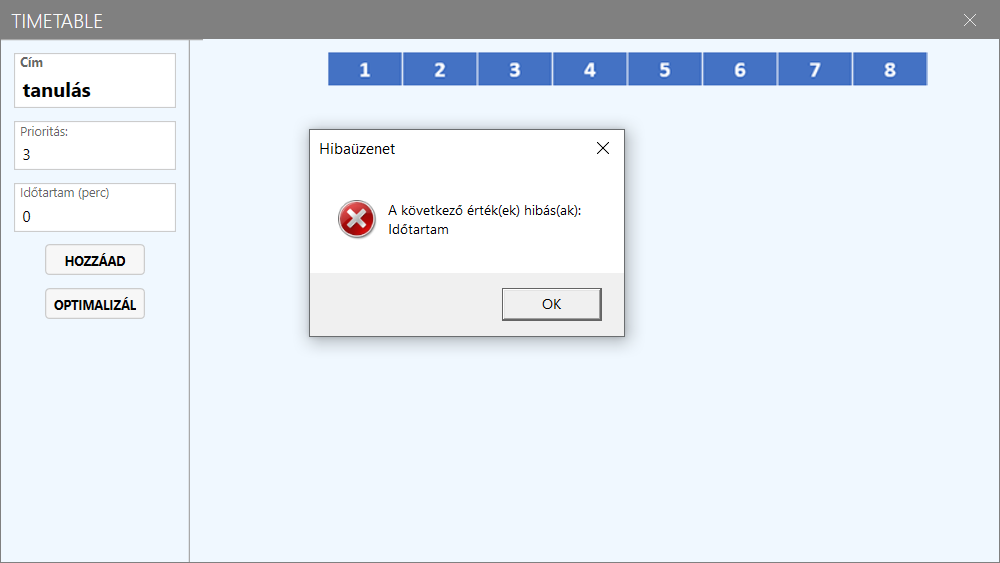
\includegraphics[width=\textwidth]{images/test/durationFault.png}
	\caption{Hibás adat megadása egy feladat hozzáada esetén}
	\label{fig:durationFault}
\end{figure}

A helyes kitöltés után egy felugró ablak jelezte a feladat sikeres hozzáadását, ezzel együtt a grafikus ábrázolás is megtörtént a diagramon.

A következő hibalehetőség felmerülése egy darab feladat optimalizálása során merülhet fel. Ilyenkor szintén hibaüzenet jelzi, hogy ennek a funkciónak az elvégzéséhez több feladat hozzáadására lenne szükség (\ref{fig:notEnoughTasks}. ábra).

\begin{figure}[h!]
	\centering
	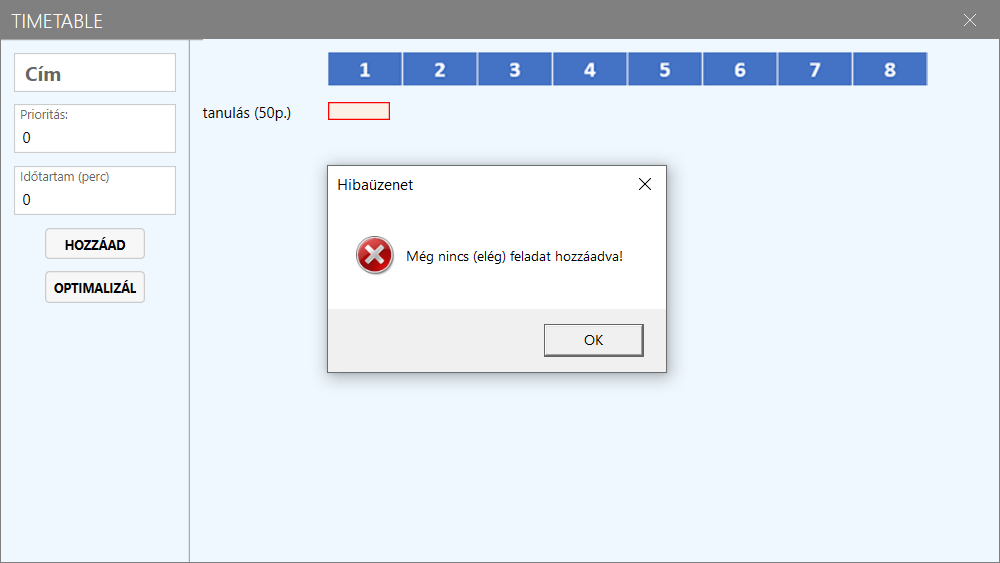
\includegraphics[width=\textwidth]{images/test/notEnoughTasks.png}
	\caption{Egy feladat esetén az ütemezés nem lehetséges}
	\label{fig:notEnoughTasks}
\end{figure}

A szemléltetés kedvéért ezek után hozzáadtam hosszabb és rövidebb tevékenységeket is, több különböző prioritással. 

\begin{figure}[h!]
	\centering
	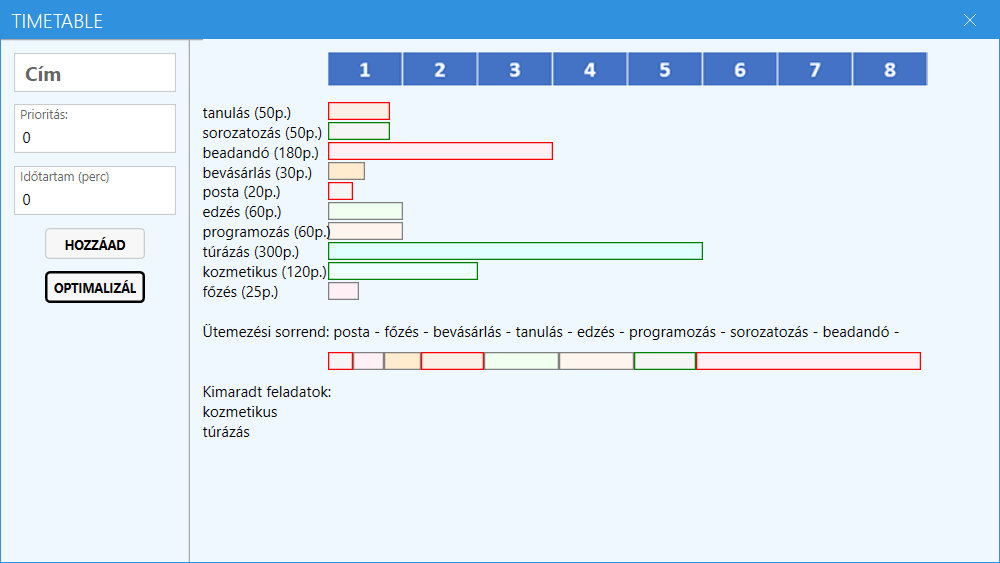
\includegraphics[width=\textwidth]{images/test/result1.png}
	\caption{Az 1. teszteset eredménye}
	\label{fig:result1}
\end{figure}

Végeredményben, mikor az optimalizálás és az ütemezés is lefutott, megjelent az előállított ütemterv, amely \aref{fig:result1}. ábrán látható. Megfigyelhető, hogy kettő feladat volt, ami már nem fért bele az ütemtervbe, mindkettő alacsony piroritással és hoszabb időtartammal rendelkezve. Ezeket a tevékenységeket külön jelzi is a program számunkra. A beütemezett feladatok közül pedig előre került egy magas prioritású feladat, követve azt egy közepes prioritásúval, amely rövid időtartama miatt is kerülhetett ennyire előre. Látható, hogy az ütemterv végén szintén magas prioritású feladat kapott helyet, ezt a többi feladathoz mérten hosszabb időtartamának köszönhette.

\Section{Teszteset 2.}

A második tesztesetben az előzőleg definiált tevékenységek újbóli megadása mellett, arra esett a választásom, hogy két feladat adatán módosítsak, megfigyelve, hogy a program az első tesztnél mennyivel különb eredményt ad. Az egyik a sorozatozás lett, amelynél ezúttal nem alacsony, hanem közepes prioritást választottam, az időtartamot meghagyva ugyanolyannak. A másik változás a beadandónál történt, itt a prioritást hagytam meg magas szinten, viszont az időtartamot jelentősen csökkentettem, az előző 3 óráról 30 percre. Így végeztem el az optimalizálást, ami \aref{fig:result1-2}. ábrán látható eredményt adta.

\begin{figure}[h!]
	\centering
	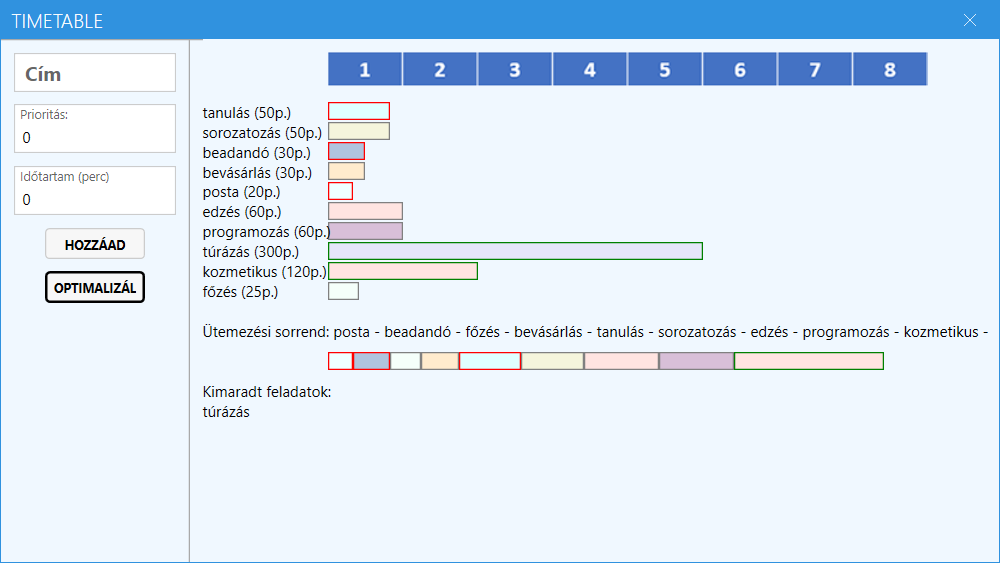
\includegraphics[width=\textwidth]{images/test/result1-2.png}
	\caption{Az 1. teszteset adatainak módosítása utáni eredmény}
	\label{fig:result1-2}
\end{figure}

Ami egyből feltűnhet az az, hogy az ütemtervből kimaradt feladatoknál már csak egy tevékenység szerepel, az előző kettőhöz képest. Ez evidens lehet, hiszen a beadandó időtartama jelentősen csökkent, így felszabadítva több helyet az időkeretben. A másik változás, hogy egyből két magas prioritású feladattal kezdődik az ütemterv, ebből a második az a beadandó írása, amely utolsó helyről került az elsők közé. A sorozatnézésnél is megfigyelhető a változás mértéke. A mostmár magasabb prioritásának köszönhetően, az ütemező hamarabbi időpontra ütemezte a sorban, megelőzve az edzés és a programozás tevékenységeket.

\Section{Teszteset 3.}

A harmadik példában már csak öt tevékenységet adtam meg, amelyek összideje 245 perc volt, azaz kicsit több, mint 4 óra. Az elvárt eredmény itt az volt, hogy ne maradjon ki feladat az ütemtervből, hiszen az időkeretbe belefér az összes feladat, de az ütemezett sorrendre nézve egy hatékony időbeosztás látszódjon. Ezt teljesítette is a program, a két magas prioritású tevékenységet ütemezte előre, kezdve a rövidebb időtartamúval. Ezt követően a közepes prioritású főzést megelőzte az alacsony prioritással rendelkező séta, köszönhetően annak, hogy arra fele annyi időt szántunk. Kimaradt feladatot nem jelzett a program (\ref{fig:result2}. ábra).

\begin{figure}[h]
	\centering
	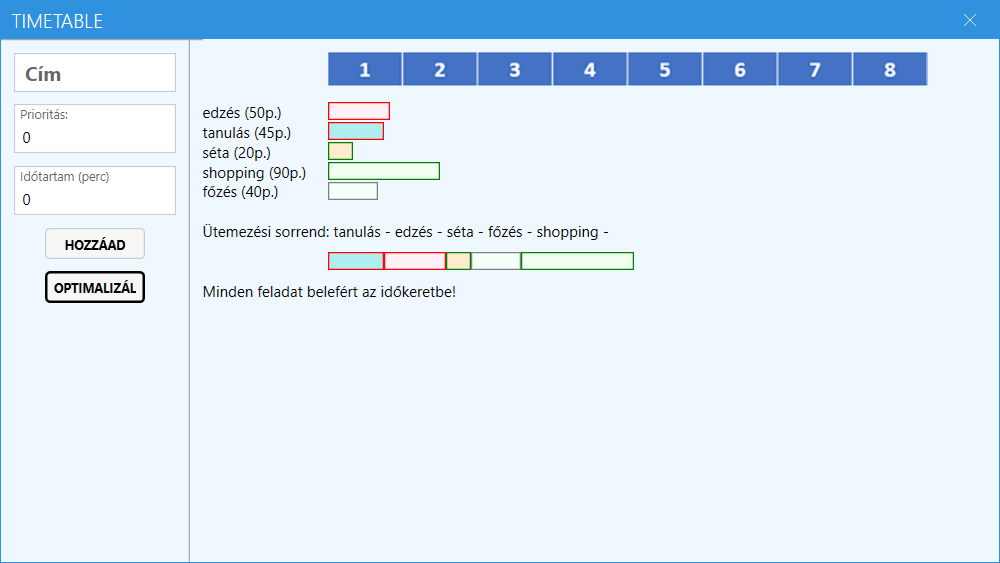
\includegraphics[width=\textwidth]{images/test/result2.png}
	\caption{Időkeretet túl nem haladó tevékenységek ütemezése}
	\label{fig:result2}
\end{figure}

\Section{Bővítési lehetőségek}

A szakdolgozatom olyan ütemezés és optimalizálás bemutatására szolgál, amely segít a mindennapi életben a teendők hatékony beütemezésében, ezáltal az időspórolásban, produktívabb életvitelben, mindezt diagramokon szemléltetve.

Az alkalmazásban még számtalan bővítési lehetőség van.
A továbbfejlesztés során lehetőség lenne például nem csak egy 8 órányi időkeretben történő ütemezésre, hanem akár heti szintű megvalósításra is. Továbbá, lehetne fix időpontban történő események megadását is lehetővé tenni, mint például egy fodrászat, fogászat vagy akár egy megbeszélt találkozó, hogy aztán az ütemező ezeket is figyelembe tudja venni.
Feladatok hozzáadásánál is számottevő bővítési lehetőség szóba jöhet, mint például:
\begin{itemize}
\item a prioritástartomány növelése,
\item színválasztás a grafikus megjelenítéshez,
\item több felhasználó hozzárendelése,
\item egyéb adatok (pl. feladat létrehozásának időpontjának) hozzárendelése,
\item helyadatok megadása,
\item sürgős feladatok jelölése a miharabbi beütemezéshez.
\end{itemize}
Mindemellett törlési funkció, heti összesítés, lekérdezések készítése is bővíthetné a program funkcionalitását.

\Chapter{Összefoglalás}

A szakdolgozatomban egy ütemező alkalmazást valósítottam meg, amely egy optimális időbeosztás elérését segíti.

A kidolgozás során áttekintettem és összehasonlítottam olyan módszereket és alkalmazásokat, amelyeket a hatékonyságnövelés céljából hoztak létre. Ennek segítségével következtettem azokra a tényezőkre, amelyeknek figyelembevétele elengedhetetlen volt a megfelelő eredmény kialakítása érdekében.
Így esett a választásom a feladatokhoz tartozó prioritás és időtartam értékekre, valamint ezek hányadosaira.

A specifikáció során összegyűjtöttem, hogy milyen adatokat kell majd kezelnie az alkalmazásnak. Ezt követően megterveztem az alkalmazás felhasználói felületét, és leírtam annak elemeit, használati módját.

Az ütemezési probléma kidolgozásához különböző algoritmusokat, módszereket és szabályokat vizsgáltam meg, amelyek az ütemezéssel és optimalizálással kapcsolatos problémákkal foglalkoznak, megoldásokat adnak rájuk. A vizsgálataim alapján végül a hátizsák feladatként emlegetett optimalizálási probléma algoritmusát használtam fel a megvalósítás során, mivel a programom ütemezési problémájához ez illeszkedett a legjobban.

A tervezésnél ismertettem a felhasznált technológiákat, amelyek segítségemre voltak az alkalmazás elkészítésében, valamint összeállítottam a feladatok és hozzá kapcsolódó műveletek modelljét.

Az implementáció során még inkább elmélyedtem a C\# sajátosságaiban, valamint megismerkedtem az \texttt{ItemsControl} és \texttt{Canvas} használatával. Ezek segítségemre voltak abban, hogy a feladatokat és az ütemtervet vizuális formában szemlélteni tudjam.
Az ütemezés eredményének megjelenítéséhez a programban az ábrát téglalap és szöveges felirat elemekből készítettem el saját implementációként.

Végeredményben sikerült egy olyan alkalmazást létrehoznom, amely prioritás és időtartam alapján vizsgálja meg felhasználó által megadott teendőket, hogy ezáltal egy minél hatékonyabb ütemtervet állítson elő számára, amelyet grafikus formában, egy diagramon jelenít meg.

A tesztelés során több esetet is megvizsgáltam annak érdekében, hogy megbizonyosodjak a program megfelelő működéséről. Az egyik teszteset során például egy már meglévő ütemterv feladatait használtam újra kisebb módosításokkal, hogy megfigyeljem mennyivel változik az eredmény. A végrehajtott módosítások láthatóan befolyásolták az új ütemterv alakulását, a módosítások mértékének megfelelően.

A dolgozatban többféle továbbfejlesztési lehetőséget felvetettem, közülük mindenképpen a nagyobb volumenű prioritásértékek megadását tartom fontosnak a precízebb eredmény elérése érdekében, valamint egy heti szintű megvalósítást, amelyben lehetőség nyílna fix időpontú események megadására, így a program naptárként és ütemezőként is funkcionálhatna egyszerre.

\newpage
\begin{LARGE}
\textbf{Summary}
\end{LARGE}
\vskip 1cm

In my thesis I implemented a scheduling application which aim is to help to create an optimized schedule for its users.

First, I reviewed and compared different methods and applications that were developed to increase efficiency. In doing so, I identified the factors that were essential to take into account in order to achieve a proper outcome. So I chose the priority and duration values defined for the tasks, and their quotients as these factors.

During specification I collected the data needed for my application.
In a further step, I have designed and described the elements and mechanics of the user interface.

To define the scheduling problem I studied various algorithms, methods and rules that address and/or solve scheduling and optimization problems. Eventually, I decided to use the algorithm of the backpack problem during the implementation as this algorithm suited the scheduling and optimization problem of my program the most.

During the design, I described the used technology, which helped me create the application. After, I defined the managed data as a class with their related methods. 

In the implementation phase, I got to learn even more about C\# and became familiar with using \texttt{ItemsControl} and \texttt{Canvas}. These classes helped me to represent the tasks and the schedule in a visual form.
The display of the results is a custom implementation, which based on the drawing of rectangles and font rendering.

Ultimately, I was able to create an application that examines the tasks defined by users on the basis of priority and duration, in order to create the most efficient schedule possible and then display it on a diagram.

During testing, I examined some cases to make sure the program was working properly. In one test case, for example, I reused the tasks of an existing schedule with minor modifications to observe how much different the new schedule would be from the original one. The changes clearly affected the outcome of the new schedule, in line with the extent of the modifications.

In the dissertation I proposed several possibilities for further development. I find it very important to specify a higher volume for priority values in order to achieve a more precise result and to create a weekly implementation where users can specify fixed time events so that the application can function as a calendar as well as a scheduler.


\clearpage

\addcontentsline{toc}{chapter}{Irodalomjegyzék}
\bibliographystyle{plain}
\bibliography{dolgozat.bib}

\newpage

\pagestyle{empty}

\noindent \textbf{\Large CD Használati útmutató}

\vskip 1cm

Ennek a címe lehet például \textit{A mellékelt CD tartalma} vagy \textit{Adathordozó használati útmutató} is.

Ez jellemzően csak egy fél-egy oldalas leírás.
Arra szolgál, hogy ha valaki kézhez kapja a szakdolgozathoz tartozó CD-t, akkor tudja, hogy mi hol van rajta.
Jellemzően elég csak felsorolni, hogy milyen jegyzékek vannak, és azokban mi található.
Az elkészített programok telepítéséhez, futtatásához tartozó instrukciók kerülhetnek ide.

A CD lemezre mindenképpen rá kell tenni
\begin{itemize}
\item a dolgozatot egy \texttt{dolgozat.pdf} fájl formájában,
\item a LaTeX forráskódját a dolgozatnak,
\item az elkészített programot, fontosabb futási eredményeket (például ha kép a kimenet),
\item egy útmutatót a CD használatához (ami lehet ez a fejezet külön PDF-be vagy MarkDown fájlként kimentve).
\end{itemize}

\newpage

\begin{LARGE}
	\textbf{Köszönetnyilvánítás}
\end{LARGE}


\end{document}
